\chapter{Algoritmo}\label{cap:algoritmo}

O algoritmo proposto nessa pesquisa é baseado no algoritmo "\textit{Watershed Algorithm Based On Connected Components}", apresentado na tese xxxx, o qual trata-se de uma variação da técnica de \textit{watershed} com resultados de segmentação considerados bastante satisfatórios além da menor complexidade computacional com relação à abordagem tradicional \textit{watershed}.

\section{\textit{Watershed}}\label{sec:watershed}
\textit{Watershed} é uma técnica de segmentação bastante eficiente e poderosa. Tal técnica tem como vantagem gerar sempre resultados com contornos fechados e bem definidos, o que é de grande importância para o processo de segmentação de imagens. Além disso, comparada a outras técnicas de segmentação, apresenta menor complexidade computacional.

Duas abordagens são bastante utilizadas para explicar a ideia básica do \textit{watershed} na segmentação de imagens. 
A primeira, denominada "\textit{flooding based watershed}", trata a imagem em níveis de cinza com uma paisagem formada por vales, onde encontram-se os mínimos locais. Considerando um processo de inundação com a água subindo a partir de cada um dos vales, serão construídas barragens nos pontos de encontro da água oriunda de dois vales distintos, chamadas de \textit{watersheds}. Essas barragens, portanto, são interpretadas como bordas entra diferentes regiões da imagem. 

% Figura
	\begin{figure}[!htb]
       \begin{center}  
          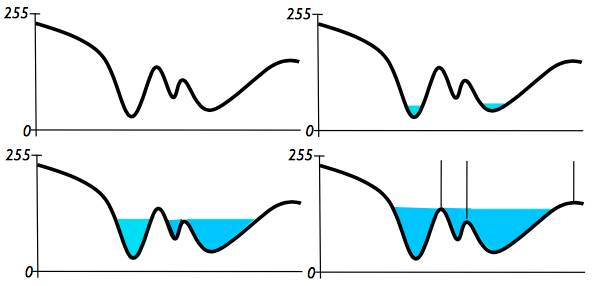
\includegraphics[width=0.8\columnwidth]{img/abordagem_flooding.jpg}
           \caption{\label{fig:abordagem_flooding}Abordagem "\textit{flooding based watershed}".}
           % \vspace{2.0em}
       \end{center}
   \end{figure} 


A outra abordagem, denominada "\textit{rainfalling based watershed}" trata a imagem em níveis de cinza da mesma forma que a primeira, porém o fluxo de água ocorre a partir de gotas de água que ao incidirem em qualquer ponto da superfície escorrerão para um determinado vale, onde encontra-se um mínimo local. O conjunto de pontos para os quais a gota de água escorre para o mesmo local é interpretada como uma região e os limites entre duas regiões adjacentes,  interpretados como bordas, são as \textit{watersheds}.

% Figura 
	\begin{figure}[!htb]
       \begin{center}  
          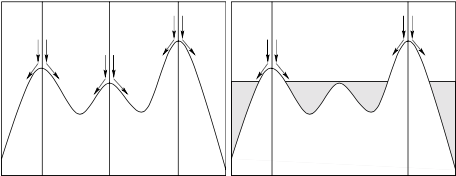
\includegraphics[width=0.8\columnwidth]{img/abordagem_rainfalling.jpg}
           \caption{\label{fig:abordagem_rainfalling}Abordagem "\textit{rainfalling based watershed}".}
           % \vspace{2.0em}
       \end{center}
   \end{figure} 
	

Ambas abordagens tratam da mesma ideia básica por trás da técnica, sendo duas formas diferentes de ilustrar seus funcionamento sobre os quais diferentes algoritmos são propostos.

Um dos principais problemas relacionados à abordagem tradicional do \textit{watershed} é o problema de \textit{over-segmentation}. Para reduzir esse problema, diversas variações de algoritmos baseados na técnica de \textit{watershed} foram implementados, tal qual o algoritmo utilizado nessa pesquisa que será explicado detalhadamente na seção \ref{sec:alg} do capítulo \ref{cap:algoritmo}. Assim as diferenças entre o algoritmo proposto e o tradicional, como o implementado na biblioteca OpenCV, apresentada na seção \ref{sec:opencv} do capítulo \ref{cap:ferramentas}, conduzirão a uma análise comparativa entre os resultados obtidos por meio de cada um deles.

\section{\textit{Watershed Algorithm Based On Connected Components}}
Destacam-se as seguintes características entre este algoritmo e a abordagem tradicional \textit{watershed} que demonstram sua maior eficiência:

% \section{Características}
\begin{itemize}
    \item Fila FIFO ao invés de fila hierárquica - algoritmo tradicional - que requer sequências de acesso à memória não uniformes;
    \item Estrutura de dados mais simples; e
    \item Menor tempo de execução.
\end{itemize}    

Este algoritmo tem como princípio conectar cada \textit{pixel} (componente), caso este não seja o mínimo local, ao menor \textit{pixel} vizinho. Todos os \textit{pixels} direcionados para o mesmo mínimo local formam um segmento e são, portanto, rotulados da mesma forma.

% Figura
	\begin{figure}[!htb]
       \begin{center}  
          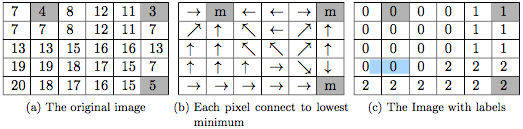
\includegraphics[width=0.8\columnwidth]{img/connected_components.jpg}
           \caption{\label{fig:connected_components}Ilustração do funcionamento da técnica \textit{Watershed Based On Connected Components}.}
           % \vspace{2.0em}
       \end{center}
   \end{figure}

\section{Implementação do Algoritmo}\label{sec:alg}

O algoritmo de segmentação proposto nessa pesquisa, assim como os demais algoritmos baseados na técnica de segmentação por \textit{watershed}, segue a estrutura apresentada na Figura \ref{fig:diagrama_blocos_algoritmo}. A imagem original passa por uma etapa de pré-processamento, em que diferentes procedimentos são realizados. Após a etapa de pré-processamento, a imagem é segmentada pela técnica \textit{watershed} e seu resultado pode ser processado, na etapa de pós-processamento, a fim de corrigir algumas falhas geradas pelo processo de segmentação para, finalmente, obter a segmentação como resultado final.
Todas as etapas serão explicadas nas próximas seções de acordo como foram implementadas no algoritmo proposto por essa pesquisa.

% Figura
	\begin{figure}[!htb]
       \begin{center}  
          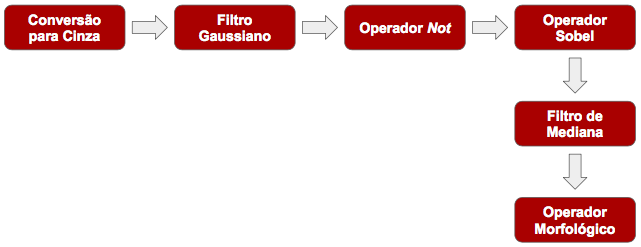
\includegraphics[width=0.7\columnwidth]{img/diagrama_blocos_preprocessamento.jpg}
           \caption{\label{fig:diagrama_blocos_algoritmo}Diagrama de blocos do algoritmo de segmentação dessa pesquisa.}
           % \vspace{2.0em}
       \end{center}
   \end{figure} 

\subsection{Pré-Processamento}
A etapa de pré-processamento tem como objetivo preparar a imagem que será utilizada na segmentação efetivamente. Para isso alguns procedimentos são realizados com o objetivo de retirar ruídos e realçar bordas para facilitar o processo de segmentação a fim de obter um resultado mais eficiente. Além disso, assim como a etapa de pós-processamento, esta etapa visa diminuir o problema de \textit{over-segmentation}, o qual tende a ocorrer quando aplica-se a técnica de \textit{watershed}.
A ordem em que esses procedimentos ocorrem nesta etapa consta na estrutura apresentada pela Figura \ref{fig:diagrama_blocos_preprocessamento}.

% Figura
	\begin{figure}[!htb]
       \begin{center}  
          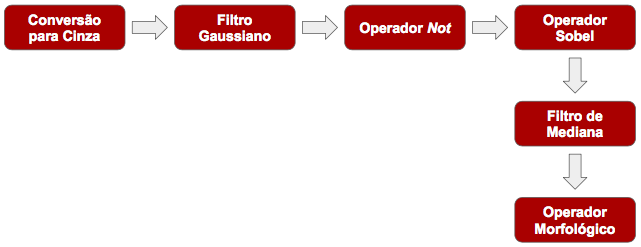
\includegraphics[width=0.8\columnwidth]{img/diagrama_blocos_preprocessamento.jpg}
           \caption{\label{fig:diagrama_blocos_preprocessamento}Diagrama de blocos da etapa de pré-processamento.}
           % \vspace{2.0em}
       \end{center}
   \end{figure}

\subsection*{Conversão para Cinza}
Um dos procedimentos realizados na etapa de pré-processamento é a conversão da imagem original colorida para a imagem em níveis de cinza. Utiliza-se a quantização em 256 níveis de cinza (8 bits), onde o nível zero representa o preto e o nível 255, o branco.
O objetivo dessa conversão é ...   

\subsection*{Operador \textit{Not}}

\subsection*{Operador Sobel}
Operador de detecção de bordas, que se baseia no operador gradiente. Esse operador é utilizado sobre a imagem resultante do operador \textit{not} com a finalidade de gerar uma imagem com as bordas detectadas brilhantes em um fundo (\textit{background}) mais escuro.

Computa-se os gradientes horizontal, \textit{Gx}, e vertical, \textit{Gy}, considerando uma janela de tamanho 3, isto é, \textit{3 x 3 pixels}, e calcula-se uma aproximação do gradiente em cada ponto da seguinte forma:

% Equação
\[G = |G_{x}| + |G_{y}|\]

% Código

\subsection*{\textit{Thresholding}}
Essa técnica de segmentação, já explicada na seção \ref{sec:alg_thresholding} do capítulo \ref{cap:algoritmos}, é aplicada sobre a imagem gradiente resultante do transformação morfológica. Seu objetivo é remover pequenas variações em regiões homogêneas e evitar a formação de diversas regiões, isto é, o problema de \textit{over-segmentation}. Dessa forma, o valor do \textit{threshold} é determinado como o mínimo local e todos os valores de gradiente menores que esse \textit{threshold} são estabelecidos também como o mínimo local.
Cada imagem demanda um valor de \textit{threshold} ideal, o qual não é fácil de ser encontrado. Para valores baixos de \textit{threshold}, as bordas podem se tornar muito largas, enquanto que para valores altos, as bordas podem não ser detectadas.
Assim, o ajuste pelo usuário se faz necessário a fim de que se possa obter a segmentação mais eficiente para uma dada imagem. Para isso, na interface do aplicativo proposto como produto final dessa pesquisa, será implementado alguma ferramenta que possibilite este ajuste.

\subsection*{Filtro de Mediana}
O objetivo do filtro de mediana é a redução ou, até mesmo, a remoção de ruídos das imagens, a fim de suavizá-las e torná-las mais tratáveis para o processo de segmentação. O filtro de mediana é eficaz para o tratamento de ruídos impulsivos, como o ruído Gaussiano (aleatório) e, principalmente, o ruído sal e pimenta, em que os \textit{pixels} ruidosos assumem os valores máximos e mínimos da imagem.
Para a implementação do filtro de mediana, considera-se uma imagem com \textit{n x m pixels} e um filtro com janela de \textit{k x k pixels}, onde \textit{k < n e k < m}. Em casa janela considerada na imagem, o valor de cada \textit{pixel} é substituído pelo valor da mediana da mesma janela. No algoritmo, usa-se \textit{k = 3} e o funcionamento do filtro pode ser entendido na Figura \ref{fig:filtromediana}.

% Figura
	\begin{figure}[!htb]
       \begin{center}  
          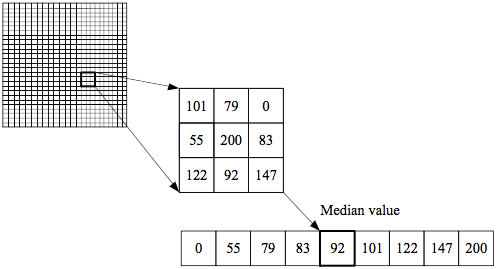
\includegraphics[width=0.8\columnwidth]{img/filtromediana.jpg}
           \caption{\label{fig:filtromediana}Ilustração do funcionamento do filtro de mediana.}
           % \vspace{2.0em}
       \end{center}
   \end{figure}
   
% Código

\subsection*{Operador Morfológico}
Utilizado sobre o resultado do operador Sobel, o operador morfológico funciona como uma técnica de realce a fim de enfatizar as bordas da imagem. 
Existem duas operações morfológicas básicas:
% \section{Operações morfológicas básicas}
\begin{itemize}
    \item Erosão; e
    \item Dilatação.
\end{itemize}    

A biblioteca OpenCV fornece 5 transformações morfológicas baseadas nessas duas operações básicas:
% \section{Transformações morfológicas}
\begin{itemize}
    \item \textit{Opening};
    \item \textit{Closing};
    \item \textit{Morphological Gradient};
    \item \textit{Top Hat}; e 
    \item \textit{Black Hat}.
\end{itemize} 

No algoritmo utiliza-se apenas a transformação \textit{closing}, a qual é útil para o fechamento de bordas, removendo pequenos buracos que possam ter sido gerados nos procedimentos anteriores.

% Equação
\[dst = close(src, element) = erode(dilate(src, element))\]


\subsection{Segmentação por Técnica Baseada em \textit{Watershed}}
Dentre as duas principais abordagens da técnica de \textit{watershed} mencionadas na seção \ref{sec:watershed} do capítulo \ref{cap:algoritmo}, optou-se pela abordagem "\textit{rainfalling based watershed}" a fim de servir como base para a implementação da etapa de segmentação implementada neste algoritmo. Essa etapa é composta por três passos (\textit{steps}). 

\subsection*{\textit{Step 1}}
% Explicar 
% Código 
 
\subsection*{\textit{Step 2}}
% Explicar 
% Código 

\subsection*{\textit{Step 3}}
% Explicar 			
% Código 

\subsection{Pós-Processamento}
Após as etapas de pré-processamento e segmentação, ainda podem ser necessárias algumas correções relacionadas ao problema de \textit{over-segmentation}. É comum que tenhamos diferentes segmentos que fazem parte de uma mesma região. Para tanto pode-se utilizar algum método de  agrupamento para mesclar esses segmentos a fim de melhorar a qualidade da segmentação.